\documentclass[a4paper, 11pt, ngerman, fleqn]{article}
\usepackage[latin1]{inputenc}
\usepackage{babel}
\usepackage{ngerman}
\usepackage{coordsys,logsys,color}
\usepackage{german,fancyhdr}
\usepackage{hyperref}
\usepackage{texdraw}
\usepackage{listings}
\usepackage{graphicx}
\input{txdtools}

\NeedsTeXFormat{LaTeX2e}
\ProvidesPackage{hyperref}
\definecolor{darkblue}{rgb}{0,0,.6}
\hypersetup{pdftex=false, colorlinks=true, breaklinks=true, linkcolor=darkblue, menucolor=darkblue, pagecolor=darkblue, urlcolor=darkblue, citecolor=darkblue}

\pagestyle{fancy}

\renewcommand{\familydefault}{cmss}

\definecolor{fgcgray}{rgb}{0.4, 0.4, 0.4}
\definecolor{warning}{rgb}{0.9, 0.1, 0.0}
\definecolor{bgctitle}{rgb}{0.5, 0.5, 0.5}
\definecolor{fgctitle}{rgb}{0.95, 0.95, 0.95}
\newcommand{\titlefont}[1]{\textcolor{fgctitle}{\fontfamily{cmss}\fontseries{bx}\fontshape{n}\fontsize{20.48}{0pt} \selectfont #1}}
\newcommand{\inversetitlefont}[1]{\textcolor{bgctitle}{\fontfamily{cmss}\fontseries{bx}\fontshape{n}\fontsize{20.48}{0pt} \selectfont #1}}

\addtolength{\oddsidemargin}{-1.0cm}
\addtolength{\evensidemargin}{-1.0cm}
\addtolength{\headwidth}{2.0cm}
\addtolength{\textwidth}{2.0cm}

\setlength{\parindent}{0cm}

\renewcommand{\labelitemi}{$\circ$}
\renewcommand{\labelitemii}{$\diamond$}

\newcommand{\spaceline}[1][8pt]{\vskip #1}
\newcommand{\comment}[1]{\spaceline[5pt] \textcolor{fgcgray}{\scriptsize #1} \spaceline[15pt]}
\newcommand{\attrname}[1]{\textcolor{fgcgray}{\scriptsize #1}}


\makeatletter

\newcommand*{\project}[1]{\gdef\@project{#1}}
\newcommand*{\version}[1]{\gdef\@version{#1}}
\newcommand*{\home}[1]{\gdef\@home{#1}}
\newcommand*{\homeref}[1]{\gdef\@homeref{#1}}
\newcommand*{\prerequisite}[1]{\gdef\@prerequisite{#1}}
\newcommand*{\prerequisiteref}[1]{\gdef\@prerequisiteref{#1}}

\def\@maketitle{
  %\begin{titlepage}
  \begin{center}
    \colorbox{bgctitle}{
      \parbox{\textwidth}{
        \spaceline
        \centering{\titlefont{\@title}}
        \par
        \spaceline
      }
    }
    \colorbox{white}{
      \parbox{\textwidth}{
        \spaceline
        \centering{\inversetitlefont{\@project}}
        \par
        \spaceline
      }
    }
  \end{center}
  \spaceline[1.5em] {
    \begin{flushright}
    \begin{tabular}[t]{rl}
      \attrname{Projekt:} & \@project ~ \@version \\
      %\attrname{Voraussetzung:} & \href{\@prerequisiteref}{\@prerequisite} \\
      \attrname{Autoren:} & \@author \\
      %\attrname{Home:} & \href{\@homeref}{\@home} \\
      %\attrname{letzte "Anderung:} & \@date
    \end{tabular}
    \end{flushright}
    \par
  }
  \spaceline[5.5em]
  %\end{titlepage}
}

\setcounter{secnumdepth}{4}
\setcounter{tocdepth}{4}
	 
\newcounter{subsubsubsection}[subsubsection]
\def\subsubsubsectionmark#1{}
\def\thesubsubsubsection{\thesubsubsection .\arabic{subsubsubsection}}
\def\subsubsubsection{\@startsection{subsubsubsection}{4}{\z@}{-3.25ex plus -1 ex minus -.2ex}{1.5ex plus .2ex}{\normalsize\bf}}
\def\l@subsubsubsection{\@dottedtocline{4}{4.8em}{4.2em}}

\makeatother

\everytexdraw{
  \drawdim cm \linewd 0.01
  \arrowheadtype t:T
  \arrowheadsize l:0.2 w:0.2
  \setgray 0.5
}

\newcommand{\xheight}{0.6}
\newcommand{\xlength}{0.6}
\newcommand{\yheighta}{1.0}
\newcommand{\yheightb}{0.8}
\newcommand{\yheightc}{0.6}
\newcommand{\yheightd}{0.5}
\newcommand{\yheighte}{0.4}
\newcommand{\yheightf}{0.35}

\newcommand{\xhline}{\rlvec({\xlength} 0)}
\newcommand{\xharrow}{\ravec(0.7 0)}
\newcommand{\xnext}{%\rlvec(0.05 0) \lpatt(0.04 0.04) \rlvec(0.15 0) \lpatt()
}

\newcommand{\xtext}[3][\xheight]{
  \bsegment
    \bsegment
      \setsegscale 0.5
      \textref h:L v:C  \htext({\xheight} -0.1){#3}
    \esegment
    \setsegscale 0.5 \lvec(0 #1)
    \setsegscale 1
    \rlvec(#2 0) \rlvec(0 -#1) \rlvec(-#2 0) \lvec(0 0)
    \savepos(#2 0)(*@x *@y)
  \esegment
  \move(*@x *@y)
}

\newcommand{\bxtext}[3][\xheight]{
  \setgray{0.1}
  \linewd{0.026}
  \xtext[\xheight]{#2}{#3}
  \linewd{0.01}
  \setgray{0.5}
}

\newcommand{\xstartpage}{\bxtext{2.1}{Startseite}}
\newcommand{\xmainpage}{\bxtext{2.3}{Hauptseite}}
\newcommand{\xusermenu}{\bxtext{2.9}{Benutzermenu}}
\newcommand{\xgamelist}{\bxtext{2.2}{Spieleliste}}
\newcommand{\xportfolio}{\bxtext{2.0}{Portfolio}}
\newcommand{\xaccount}{\xtext{3.8}{Kennung per \textsl{eMail}}}


\begin{document}
  \lhead{\sc{Pflichtenheft Scalomator}}
%\cfoot{-~\thepage~-}
\title{Pflichtenheft}
\project{Scalomator}
\version{}
%\prerequisite{Lastenheft}
%\prerequisiteref{http://www.stefan-baur.de/downloads/Lastenheft.pdf}
\author{Nils Foken, Christian Krause, Peter Kossek}
\home{www.stefan-baur.de}
\homeref{http://www.stefan-baur.de/cs.se.pflichtenheft.html}

\maketitle

%\textcolor{warning}{Diese Datei zeigt NUR ein Beispiel eines Pflichtenheftes!}\\
%\textcolor{warning}{Verwendung auf eigene Gefahr!}
%\thispagestyle{empty}
%~
%\newpage
%\tableofcontents
 \newpage
  \tableofcontents \newpage
  \section{Zielbestimmungen}
\textbf{Scalomator} ist ein Computerprogramm, welches die Ausf�hrung endlicher Automaten auf eine Eingabe simuliert. Hierbei sollen sowohl deterministische endliche Automaten (deterministic final automaton, DFA) als auch nichtdeterministische endliche Automaten (nondeterministic finite automaton, NFA) simuliert werden k�nnen.
\\\\
Das Programm soll der Unterst�tzung der Ausbildung von Studenten der Studienrichtung Informatik an der Staatlichen Studienakademie Leipzig im Fachgebiet der theoretischen Informatik dienen.
\\\\
Ein \textbf{Automat} ist in der Informatik das Modell eines digitalen, zeitdiskreten Rechners. Ob es m�glich oder sinnvoll ist, eine solche Maschine tats�chlich zu bauen, ist dabei zun�chst unerheblich. Die Vereinfachung der F�higkeiten erlaubt es, das Verhalten eines Automaten leichter zu verstehen und zu vergleichen.
\\\\
Das grunds�tzliche Verhalten eines Automaten ist immer gleich: Dem Automaten wird von au�en eine Eingabe als Folge von Zeichen vorgelegt. Der Automat befindet sich in einem Zustand. Jedes Mal, wenn ein Eingabezeichen eintrifft, kann sich abh�ngig vom Eingabezeichen und dem gegenw�rtigen Zustand ein neuer Zustand, der Folgezustand, einstellen (Zustands�bergang oder Transition). Man kann die Menge der m�glichen Zustands�berg�nge, die das Verhalten des Automaten definiert, als das Programm des Automaten verstehen.
\\\\
Wenn der Folgezustand durch den gegenw�rtigen Zustand und das Eingabezeichen immer eindeutig gegeben ist, dann spricht man von einem \textbf{deterministischen Automaten}. Allgemein aber kann man auch einen Spielraum (Freiheitsgrade) f�r die Zustands�berg�nge zulassen. Der Automat darf dann auf dasselbe Paar von Zustand und Eingabezeichen unter mehreren m�glichen Kandidaten einen Folgezustand willk�rlich w�hlen. Dann spricht man von einem \textbf{nichtdeterministischen Automaten}. Der Nichtdeterminismus ist dann willkommen, wenn man das Verhalten der Umgebung modellieren m�chte, das man nicht v�llig genau kennt (don't know), oder wenn man M�glichkeiten f�r verschiedene Implementierungen offenlassen m�chte (don't care).
\\\\
Ein Automat hei�t endlich, wenn die Menge der Zust�nde, die er annehmen kann, endlich ist. Ein \textbf{endlicher Automat} ist ein Spezialfall aus der Menge der Automaten. Ein Zustand speichert die Information �ber die Vergangenheit, d.h. er reflektiert die �nderungen der Eingabe seit dem Systemstart bis zum aktuellen Zeitpunkt. Ein Zustands�bergang zeigt eine �nderung des Zustandes des endlichen Automaten und wird durch logische Bedingungen beschrieben, die erf�llt sein m�ssen, um den �bergang zu erm�glichen. Eine Aktion ist die Ausgabe des endlichen Automaten, die in einer bestimmten Situation erfolgt. 
\\\\
Ein endlicher Automat wird definiert durch ein 5-Tupel $(\Sigma, S, s_0, \delta, E)$, wobei:
\begin{itemize}
\item[$\Sigma$] ist das Eingabealphabet (eine endliche nicht leere Menge von Symbolen),
\item[$S$] ist eine endliche nicht leere Menge von Zust�nden,
\item[$s_0$] ist der Anfangszustand, $s_0\in S$,
\item[$\delta$] ist die Zustands�bergangsfunktion: $\delta: S \times \Sigma \rightarrow S$,
\item[$E$] ist die Menge von Endzust�nden, $E \subseteq S$
\end{itemize}

\subsection{Musskriterien}

\begin{itemize}
  \item Berechnungsprogramm
    \begin{itemize}
      \item Entgegennahme von Automatendefinition.
      \item Entgegennahme von Eingabewort.
      \item Berechnung der Akzeptanz des Automaten f�r dieses Eingabewort.
      \item Ausgabe der Akzeptanz (Simulationsergebnis).
    \end{itemize}
  \item Grafische Benutzeroberfl�che
    \begin{itemize}
      \item Erstellen von Automatendefinitionen durch grafische Oberfl�che.
      \item Speicherung von erstellten Automatendefinitionen auf Speichermedien.
      \item Laden von bereits erstellten Automatendefinitionen von Speichermedien.
      \item Start des Berechnungsprogramms und Anzeige des Simulationsergebnisses.
    \end{itemize}
\end{itemize}

\subsection{Wunschkriterien}

\begin{itemize}
  \item Eine Ausgabe des Simulationsablaufs.
\end{itemize}

\subsection{Abgrenzungskriterien}

\begin{itemize}
  \item Keine Simulation von Kellerautomaten oder Turingmaschinen.
\end{itemize}
 \newpage
  \section{Produkteinsatz}

%\comment{Welche Anwendungsbereiche (Zweck), Zielgruppen (Wer mit welchen Qualifikationen), Betriebsbedingungen (Betriebszeit, Aufsicht)?}

\subsection{Anwendungsbereiche}

Einzelpersonen verwenden dieses Programm zur Simulation endlicher Automaten.

%Einzelpersonen verwenden diesen Dienst zum Spielen der oben angegebenen Brettspiele mit anderen Personen der Spielgemeinschaft.
%Diese Plattform soll dem Einzelnen eine Kommunikation mit Gleichgesinnten erm�glichen,
%um so ihre Fertigkeiten im Spiel verbessern zu k�nnen.

\subsection{Zielgruppen}

Studenten, die im Bereich der theoretischen Informatik ausgebildet werden, sollen ihre Kenntnisse im Fachgebiet der Automatentheorie mittels dieses Programms vertiefen und festigen.
Zuvor per Hand ermittelte Ergebnisse k�nnen von den Studenten �berpr�ft werden.

%Personengruppen, die kurz zur Ablenkung z.B. in der Mittagspause, gerne an Fernspielen teilhaben,
%in dem sie sich Gedanken �ber bevorstehende Spielz�ge machen k�nnen.\\
%Diese Plattform ist f�r Einzelpersonen gedacht, die in ihrer knapp bemessenen Freizeit Schwierigkeiten haben,
%ihrem Hobby z.B. Schach nachzugehen oder Gegner zu finden.\\
%\\
%Es werden Basiskenntnisse in Internetnutzung vorausgesetzt. Ebenso die Spielregeln des jeweiligen Spieltyps sollten vor der
%Nutzung bekannt sein.\\
%\\
Soweit keine weiteren Sprachen integriert sind, muss der Benutzer die Verkehrssprache \textit{Englisch} zumindest verstehen.

\subsection{Betriebsbedingungen}

Dieses System soll sich bez�glich der Betriebsbedingungen nicht wesentlich von anderen Anwendungen unterscheiden.

\begin{itemize}
  \item Betriebsdauer: wenn ben�tigt
  \item wartungsfrei
\end{itemize}
 \newpage
  \section{Produktumgebung}

%\comment{Welche Software, Hardware und Orgware wird ben�tigt?}

Das Produkt ist weitgehend unabh�ngig vom Betriebssystem, sofern nachfolgende Produktumgebung gegeben ist.

\subsection{Software}

\begin{itemize}
	\item Java Runtime Environment (JRE), mindestens Version 1.6
\end{itemize}
      
\subsection{Hardware}

\begin{itemize}
	\item Computer mit grafischer Oberfl�che, auf dem eine Java Runtime Environment lauff�hig ist.
\end{itemize}

%\subsection{Orgware}

%\begin{itemize}
%  \item Gew�hrleistung der permanenten Internetanbindung
%  \item Administrator muss den Internetdienst starten und die Betriebsparameter konfigurieren
%\end{itemize}
 \newpage
  \section{Produktfunktionen}

%\comment{Was leistet das Produkt aus Benutzersicht?}

\subsection{Grafische Benutzeroberfl�che}

Die grafische Benutzeroberfl�che dient der komfortablen Erzeugung von Automatendefinitionen.

\subsubsection{Zeichnen von Graphen}

\begin{description}
\item[/F0010/]
	\textit{Zustand erstellen:} Der Benutzer legt einen neuen Zustand im Graphen an, welcher ihm als ein Kreis angezeigt wird.
	Der Kreis beinhaltet einen Text, der dem Namen des Zustands entspricht.
\item[/F0020/]
	\textit{Zustand l�schen:} Bereits erstellte Zust�nde k�nnen vom Benutzer gel�scht werden.
\item[/F0030/]
	\textit{Zustand umbenennen:} Der Name eines Zustandes muss �nderbar sein.
\item[/F0040/]
	\textit{Zustand verschieben:} Die Position des Zustands kann durch Verschieben angepasst werden.
\item[/F0100/]
	\textit{�bergang erstellen:} Zustands�bergange stellen die Aktionsm�glichkeiten 
\item[/F0110/]
	\textit{�bergang l�schen}
\item[/F0120/]
	\textit{�bergang bearbeiten}
\item[/F0200/]
	\textit{Zustand zu Startzustand erkl�ren}
\item[/F0200/]
	\textit{Zustand zu Endzustand erkl�ren}
\item[/F0200/]
	\textit{Startzustand oder Endzustand zu normalen Zustand erkl�ren}
\end{description}

\subsubsection{Dateioperationen}

\begin{description}
\item[/F0300/]
	\textit{Automatendefinition speichern}
\item[/F0310/]
	\textit{Automatendefinition laden}
\item[/F0320/]
	\textit{Neue Automatendefinition erstellen}
\end{description}

\subsubsection{Simulation}

\begin{description}
\item[/F0400/]
	\textit{Simulation ausf�hren}
\item[/F0410/]
	\textit{Simulationsergebnis anzeigen}
\end{description}


\subsection{Kommandozeilenprogramm}

Neben der grafischen Benutzeroberfl�che existiert ebenfalls ein Kommandozeilenprogramm, das �ber Parameter die Simulation eines Automaten anst��t.

\begin{description}
\item[/F1000/]
	\textit{Ausgabe einer Beschreibung der Programmparameter:} Um auf der Kommandozeile ausgef�hrt werden zu k�nnen ben�tigt das Simulationsprogramm eine Reihe von Parametern (Eingabewort, Automatendefinition, evtl. aus Datei gelesen). Diese Parameter werden mitsamt einer Beschreibung auf der Konsole ausgegeben.
\item[/F1010/]
	\textit{Ausf�hrung der Simulation:} 	
\end{description}

\subsection{Bibliothek}

Die Bibliothek ist eine separate Komponente, die unabh�ngig von der grafischen Benutzeroberfl�che operiert.
Es bietet auch die M�glichkeit, �ber die Kommandozeile gestartet zu werden und dort das Ergebnis der Simulation anzuzeigen.

\begin{description}
\item[/F2000/]
	\textit{Simulation eines endlichen Automaten}
\end{description}

%\subsection{Benutzerfunktionen}
%
%\subsubsection{Benutzer-Kennung}
%
%Ein im System registrierter Benutzer kann das System erst nutzen, wenn er angemeldet ist.
%
%\begin{description}
%  \item[/F0010/]
%    \textit{Registrieren:} Ein beliebiger Internet-Benutzer kann sich �ber die Start- bzw. Login-Seite des Systems
%    schnell und bequem registrieren lassen. Zum Registrieren sind mindestens folgende Angaben erforderlich:
%    \begin{itemize}
%      \item gew�nschte \textbf{Kennung}
%        \begin{itemize}
%          \item gew�nschter \textbf{Benutzername}
%          \item gew�nschtes \textbf{Passwort}
%        \end{itemize}
%      \item eigene bzw. private \textbf{eMail-Adresse}
%    \end{itemize}
%    Die Registrierung ist erfolgreich, wenn der \textit{Benutzername} und die \textit{eMail-Adresse}
%    innerhalb des Systems jeweils eindeutig sind. Die \textit{eMail-Adresse} wird auf ihre G�ltigkeit gepr�ft.\\
%    Mit dem erfolgreichen Abschie�en des Registrierungsvorgangs ist der neue Benutzer am System angemeldet,
%    zudem erh�lt der Benutzer automatisch via \textit{eMail} vom System seine aktuelle Kennung.
%  \item[/F0020/]
%    \textit{Anmelden:} Ein bereits registrierter Benutzer kann sich �ber die Start- bzw. Login-Seite des Systems
%    schnell und bequem anmelden \textit{(login)}. Dazu ist seine Kennung erforderlich:
%    \begin{itemize}
%      \item sein \textbf{Benutzername}
%      \item sein \textbf{Passwort}
%    \end{itemize}
%    Alternativ zum \textit{Benutzernamen} kann der Benutzer seine \textit{eMail-Adresse} angeben.
%  \item[/F0030/]
%    \textit{Abmelden:} Der angemeldete Benutzer kann sich jeder Zeit wieder vom System \textbf{abmelden} \textit{(logout)}.
%  \item[/F0040/]
%    \textit{Kennung anfordern:} Falls ein bereits registrierter Benutzer seine Kennung oder sein \textbf{Passwort vergessen}
%    haben sollte, so kann er seine korrekte Kennung �ber die Start- bzw. Login-Seite des Systems anfordern.
%    Dem Benutzer wird unter Angabe
%    \begin{itemize}
%      \item seines \textbf{Benutzernamens} oder
%      \item seiner \textbf{eMail-Adresse}
%    \end{itemize}
%    seine vollst�ndige Kennung automatisch via \textit{eMail} vom System zugesendet.
%  \item[/F0050/]
%    \textit{Passwort �ndern:} Der angemeldete Benutzer kann das Passwort seiner Kennung �ndern.
%    Das neue Passwort muss zweimal angegeben werden, wobei sich diese Angaben nicht unterscheiden d�rfen.
%    Nach erfolgreicher �nderung des Passwortes erh�lt der Benutzer automatisch via \textit{eMail} vom System seine aktuelle Kennung.
%\end{description}
%
%Der Benutzer kann seinen \textit{Benutzernamen} nicht �nderen.\\
%\\
%Im Folgenden sei der Benutzer stets am System angemeldet.
%
%\subsubsection{Pers�nliche Daten}
%
%Der Benutzer verf�gt �ber pers�nliche Daten \textit{(siehe /D010/)}, die er frei gestalten kann.
%
%\begin{description}
%  \item[/F0110/]
%    \textit{Anzeige der eigenen, pers�nlichen Daten:}
%    Der Benutzer kann sich seine pers�nlichen Daten vom System \textbf{vollst�ndig anzeigen} lassen.
%  \item[/F0120/]
%    \textit{�ndern der eigenen, pers�nlichen Daten:}
%    Der Benutzer kann seine pers�nlichen Daten aktualisieren bzw. \textbf{�ndern}.
%  \item[/F0130/]
%    \textit{Sichtbarkeit der eigenen, pers�nlichen Daten:}
%    Der Benutzer kann jeden einzelnen Eintrag seiner pers�nlichen Daten f�r die Spielgemeinschaft auf \textbf{sichtbar} bzw.
%    \textbf{unsichtbar} setzen.
%  \item[/F0140/]
%    \textit{Anzeige der pers�nlichen Daten anderer Benutzer:}
%    Der Benutzer kann sich von anderen Benutzern die pers�nlichen Daten anzeigen lassen,
%    dabei k�nnen auf unsichtbar gesetzte Eintr�ge nicht gesehen werden.\\
%    Im Gegensatz zu \textit{/F0110/} kann der Benutzer seine eigenen, pers�nlichen Daten auch auf diese Weise anzeigen lassen.
%\end{description}
%
%
%\subsubsection{Pers�nliche Konfiguration}
%
%Die Nutzungsumgebung eines Benutzers ist das Layout, das Design, aber auch diverse logische Einstellungen,
%die die individuelle Handhabung des Systems vereinfachen k�nnen.\\
%Individuell einstellbar f�r den Benutzer sind:
%\begin{itemize}
%  \item die Farbgebung
%  \item die Gliederung seiner Hauptseite \textit{(Anordnung von Men�, Spielfl�che und Spieleliste)}
%\end{itemize}
%Zudem kann der Benutzer noch einstellen, welche Informationen direkt nach dem \textit{Login} auf der Hauptseite angezeigt werden sollen.
%Pers�nliche Konfigurationen k�nnen verwaltet werden \textit{(siehe Portfolio)}.
%
%\begin{description}
%  \item[/F0210/]
%    \textit{Anzeige der pers�nlichen Konfiguration:}
%    Der Benutzer kann sich alle einstellbaren Werte seiner pers�nlichen Konfiguration seiner Nutzungsumgebung vom System \textbf{anzeigen} lassen.
%  \item[/F0220/]
%    \textit{�ndern der pers�nlichen Konfiguration:}
%    Der Benutzer kann alle einstellbaren Werte seiner pers�nlichen Konfiguration \textbf{�ndern}
%    oder die voreingestellte Konfiguration wiederherstellen.
%  \item[/F0230/]
%    \textit{Speichern der pers�nlichen Konfiguration:}
%    Der Benutzer kann seine pers�nliche Konfiguration \textbf{speichern} bzw. in seiner \textit{Portfolio} \textbf{sichern}.
%  \item[/F0240/]
%    \textit{L�schen der pers�nlichen Konfiguration:}
%    Der Benutzer kann bereits gesicherte Konfigurationen aus seiner \textit{Portfolio} \textbf{entfernen}.
%  \item[/F0250/]
%    \textit{Wiederverwenden der pers�nlichen Konfiguration:}
%    Der Benutzer kann bereits gesicherte Konfigurationen seiner \textit{Portfolio} \textbf{wiederverwenden}.
%    Beim Wechseln der Konfiguration wird das gleichzeitige Sichern der aktuellen Konfiguration angeboten.
%\end{description}
%
%\subsubsection{Pers�nliches Profil}
%
%Der Benutzer bzw. der Spieler verf�gt �ber ein pers�nliches Profil.
%Dieses kann man in zwei Teile gliederen:
%\begin{itemize}
%  \item allgemeines Profil
%    \begin{itemize}
%      \item die H�ufigkeit des Erscheinens \textit{(Treue)}
%    \end{itemize}
%  \item Profil zu jedem Spieltyp \textit{(M�hle, Dame und Schach)}
%    \begin{itemize}
%      \item die Wertung \textit{(aktuelle Spielst�rke in Form einer Zahl)}
%      \item die Anzahl der gespielten, gewonnenen, verlorenen und unentschiedenen Spiele
%      \item die Anzahl der noch offenen Spiele
%      \item die Auflistung von Auszeichnungen
%        \begin{itemize}
%          \item der beste
%          \item der schlechteste
%          \item der schnellste
%          \item der langsamste
%          \item der treueste
%          \item der bekannteste Spieler \textit{(der Woche, des Monats und des Jahres)}
%        \end{itemize}
%    \end{itemize}
%\end{itemize}
%
%Das pers�nliche Profil wird je nach Bedarf vom System automatisch aktualisiert, die Wertung wird z.B. nach dem Beenden einer Partie aktualisiert.
%
%\begin{description}
%  \item[/F0310/]
%    \textit{Anzeige des eigenen, pers�nlichen Profils:}
%    Der Benutzer kann sich sein pers�nliches Profil f�r jeden Spieltyp \textbf{anzeigen} lassen.
%  \item[/F0320/]
%    \textit{Sichtbarkeit des eigenen, pers�nlichen Profils:}
%    Der Benutzer kann jeden einzelnen Eintrag seines pers�nlichen Profils f�r die Spielgemeinschaft auf \textbf{sichtbar} bzw.
%    \textbf{unsichtbar} setzen.
%    Jedoch die Wertungen bleiben immer �ffentlich sichtbar.
%  \item[/F0330/]
%    \textit{Anzeige der pers�nlichen Profile anderer Benutzer:}
%    Der Benutzer kann sich von anderen Benutzern die pers�nlichen Profile anzeigen lassen,
%    dabei k�nnen auf unsichtbar gesetzte Eintr�ge nicht gesehen werden.\\
%    Im Gegensatz zu \textit{/F0310/} kann der Benutzer sein eigenes, pers�nliches Profil auch auf diese Weise anzeigen lassen.
%\end{description}
%
%
%\subsection{Spielfunktionen}
%
%Der angemeldete Benutzer ist in erster Linie ein Spieler.
%Dieser Spieler hat stets eine Liste von eigenen, laufenden Spielen zur Verf�gung.\\
%Ein Spieler kann nicht gegen sich selbst antreten.
%
%\subsubsection{Initialisierung}
%
%\begin{description}
%  \item[/F0410/]
%    \textit{Er�ffnung eines Spieles:}
%    Der angemeldete Benutzer kann Spiele \textbf{er�ffnen}, ohne dabei einen anderen Spieler als Gegner angeben zu m�ssen.
%    Ein er�ffnetes Spiel kann von anderen Spieleren unter dem Men�punkt \textbf{neue Spiele} angenommen werden \textit{/F0420/}.
%  \item[/F0420/]
%    \textit{Aufnahme eines Spieles:}
%    Der angemeldete Benutzer kann bereits er�ffnete Spiele \textbf{aufnehmen} \textit{/F0410/}.
%  \item[/F0430/]
%    \textit{Herausfordern eines Gegners:}
%    Der angemeldete Benutzer kann unter Angabe eines g�ltigen Benutzernamens einen anderen Benutzer zum Spiel \textbf{herausfordern}.
%  \item[/F0440/]
%    \textit{Annahme einer Herausforderung:}
%    Der angemeldete Benutzer kann eine Herausforderung zum Spiel \textit{/F0430/} \textbf{annehmen}.
%  \item[/F0450/]
%    \textit{Ablehnen einer Herausforderung:}
%    Der angemeldete Benutzer kann eine Herausforderung zum Spiel \textit{/F0430/} \textbf{ablehnen}.
%\end{description}
%
%\subsubsection{Spielverlauf}
%
%\begin{description}
%  \item[/F0510/]
%    \textit{Zugm�glichkeit:}
%    Der angemeldete Benutzer kann zu jedem Spiel einen Zug seiner Wahl gem�� der Spielregeln \textbf{ziehen}, vorausgesetzt er ist am Zug.
%  \item[/F0520/]
%    \textit{Gebot eines Unentschieden:}
%    Der angemeldete Benutzer kann gem�� den Spielregeln ein Unentschieden \textit{(remis)} \textbf{anbieten}, vorausgesetzt er ist am Zug.
%  \item[/F0530/]
%    \textit{Annahme eines Unentschieden:}
%    Der angemeldete Benutzer kann, wenn ihm ein Unentschieden angeboten wurde \textit{/F0520/}, das Unentschieden \textbf{annehmen}.
%  \item[/F0540/]
%    \textit{Ablehnen eines Unentschieden:}
%    Der angemeldete Benutzer kann, wenn ihm ein Unentschieden angeboten wurde \textit{/F0520/}, das Unentschieden \textbf{ablehnen}.
%  \item[/F0550/]
%    \textit{Aufgabe eines Spieles:}
%    Der angemeldete Benutzer kann ein laufendes Spiel \textbf{mit Aufgabe beenden}, vorausgesetzt er ist am Zug.
%  \item[/F0560/]
%    \textit{Zugbedingter Nachrichtenaustausch:}
%    Der angemeldete Benutzer kann zu jedem Zug \textbf{eine Nachricht �bermitteln}.
%\end{description}
%
%\subsection{Portfolio-Funktionen}
%
%Der Benutzer verf�gt �ber eine pers�nliche Sammel- und Dokumentenmappe,
%die mit Such-, Sortier- und Dokumentationsfunktionen versehen ist.
%Dieses Portfolio ist rein zur privaten Verwendung und deshalb nicht f�r die Spielgemeinschaft sichtbar.
%Das Portfolio erm�glicht das individuelle Dokumentieren und Sammeln im System.\\
%Der Benutzer kann grunds�tzlich alles Sammelbare in sein Portfolio aufnehmen.\\
%Zum Sammelbaren z�hlen:
%\begin{itemize}
%  \item pers�nliche Konfigurationen
%  \item andere Benutzer bzw. Spieler
%  \item bereits beendete Spiele
%  \item Nachrichten
%  \item Notizen
%\end{itemize}
%
%\begin{description}
%  \item[/F0610/]
%    \textit{Anzeige des Portfolios:}
%    Der Benutzer kann sich den Inhalt des pers�nlichen Portfolios \textbf{anzeigen} lassen.
%  \item[/F0620/]
%    \textit{Suche nach Benutzern:}
%    Der Benutzer kann mit der Suchfunktion des Portfolios nach anderen Benutzern des Systems anhand einer beliebigen Kombination
%    der folgenden Kriterien suchen:
%    \begin{itemize}
%      \item Benutzername
%      \item Bereichsangabe der Wertungen zu gegebenen Spieltyp
%    \end{itemize}
%  \item[/F0630/]
%    \textit{Suche nach Spielen:}
%    Der Benutzer kann mit der Suchfunktion des Portfolios nach bereits gespielten Spielen des Systems anhand einer beliebigen Kombination
%    der folgenden Kriterien suchen:
%    \begin{itemize}
%      \item Spieltyp \textit{(M�hle, Dame, Schach oder alle)}
%      \item Anzahl der Spielz�ge
%      \item Gewinnfarbe \textit{(Weiss, Schwarz oder unentschieden)}
%    \end{itemize}
%\end{description}
%
%\subsection{Administratorfunktionen}
%
%Der Administrator verf�gt �ber alle Benutzerfunktionen, und kann dar�berhinaus die Eigenschaften des Systems konfigurieren.
%Zudem kann der Administrator Benutzer aus dem System verbannen,
%sowie den Informationsaustausch \textit{(Instant-Messaging)} zwischen zwei Benutzern v�llig unterbinden,
%sofern diese kein Spiel am Laufen haben.
%
%\subsubsection{Systemverwaltung}
%
%\begin{description}
%  \item[/F1010/]
%    \textit{Konfiguration:}
%    Der angemeldete Administrator kann die Eigenschaften des Systems
%    \begin{itemize}
%      \item Sessiondauer eines Benutzers \textit{(Autologout)}
%      \item Welche Werbebanner auf welchen Seiten angezeigt werden sollen
%    \end{itemize}
%    konfigurieren.
%  \item[/F1020/]
%    \textit{Statistiken:}
%    Der angemeldete Administrator kann sich Statistiken
%    \begin{itemize}
%      \item Welcher Spieltyp wird am h�ufigsten verwendet
%      \item Wieviele Benutzer registrieren sich pro Tag
%      \item Wieviele Benutzer sind bzw. waren am System angemeldet
%    \end{itemize}
%    zur Benutzung des Systems anzeigen lassen.
%\end{description}
%
%\subsubsection{Benutzerverwaltung}
%
%\begin{description}
%  \item[/F1110/]
%    \textit{Einsch�nkung der Benutzer:}
%    Der angemeldete Administrator kann die Eigenschaften einzelner Benutzer unter Angabe einer zeitlichen Begrenzung einschr�nken.
%    \begin{itemize}
%      \item Er kann die M�glichkeit zum Nachrichtenaustausch \textit{(Instant-Messaging)} zweier Benutzer unterbinden.
%      \item Er kann jeglichen Kontakt zwischen zwei Benutzer unterbinden, wobei bereits er�ffnete Spiele zu Ende gespielt werden m�ssen.
%    \end{itemize}
%    Eine v�llige Einschr�nkung eines Benutzers bedeutet die Verbannung eines Benutzers aus dem System.
%    Dies ist besonders sinnvoll, wenn ein Benutzer bei einem kostenpflichtigen Account seinen Zahlungen nicht nachkommen sollte
%    \textit{(Ausblick auf Folgeversion)}.
%  \item[/F1120/]
%    \textit{Einschr�nkungen restaurieren:}
%    Der angemeldete Administrator kann die Eigenschaften einzelner Benutzer auch wieder manuell restaurieren.
%\end{description}
 \newpage
  \section{Produktdaten}

%\comment{Was speichert das Produkt (langfristig) aus Benutzersicht?}

\begin{description}
  \item[/D010/]
    \textit{Automatendefinition:} Die Struktur eines endlichen Automaten, bestehend aus Zust�nden und �bergangen, wird in einer XML-Datei gespeichert, die der folgenden Definition (Listing \ref{xsd}) gen�gt.
    
    \lstset{ %
  language=XML,                % the language of the code
  basicstyle=\footnotesize,           % the size of the fonts that are used for the code
  numbers=left,                   % where to put the line-numbers
  numberstyle=\footnotesize,          % the size of the fonts that are used for the line-numbers
  stepnumber=2,                   % the step between two line-numbers. If it's 1, each line 
                                  % will be numbered
  numbersep=5pt,                  % how far the line-numbers are from the code
  backgroundcolor=\color{white},      % choose the background color. You must add \usepackage{color}
  showspaces=false,               % show spaces adding particular underscores
  showstringspaces=false,         % underline spaces within strings
  showtabs=false,                 % show tabs within strings adding particular underscores
  frame=single,                   % adds a frame around the code
  tabsize=2,                      % sets default tabsize to 2 spaces
  captionpos=b,                   % sets the caption-position to bottom
  breaklines=true,                % sets automatic line breaking
  breakatwhitespace=false,        % sets if automatic breaks should only happen at whitespace
  title=\lstname,                   % show the filename of files included with \lstinputlisting;
                                  % also try caption instead of title
  numberstyle=\tiny,        % line number style
  escapeinside={\%*}{*)},            % if you want to add a comment within your code
  morekeywords={*,...}               % if you want to add more keywords to the set
}

\begin{lstlisting}[caption=XSD,label=xsd]
<?xml version="1.0" encoding="UTF-8"?>
<xs:schema xmlns:xs="http://www.w3.org/2001/XMLSchema"
    elementFormDefault="qualified">

  <xs:element name="finitestatemachine">
    <xs:complexType>
      <xs:sequence>
        <xs:element ref="initialstate"/>
        <xs:element ref="finalstates"/>
        <xs:element ref="transitions"/>
      </xs:sequence>
      <xs:attribute name="name" type="xs:normalizedString"/>
    </xs:complexType>
  </xs:element>

  <xs:element name="initialstate" type="xs:normalizedString"/>

  <xs:element name="finalstates">
    <xs:complexType>
      <xs:sequence>
        <xs:element maxOccurs="unbounded" ref="finalstate"/>
      </xs:sequence>
    </xs:complexType>
  </xs:element>

  <xs:element name="finalstate" type="xs:normalizedString"/>

  <xs:element name="transitions">
    <xs:complexType>
      <xs:sequence>
        <xs:element maxOccurs="unbounded" ref="transition"/>
      </xs:sequence>
    </xs:complexType>
  </xs:element>

  <xs:element name="transition">
    <xs:complexType>
      <xs:sequence>
        <xs:element ref="start"/>
        <xs:element ref="input"/>
        <xs:element ref="ends"/>
      </xs:sequence>
    </xs:complexType>
  </xs:element>

  <xs:element name="start" type="xs:normalizedString"/>

  <xs:element name="input" type="xs:normalizedString"/>

  <xs:element name="ends">
    <xs:complexType>
      <xs:sequence>
        <xs:element maxOccurs="unbounded" ref="end"/>
      </xs:sequence>
    </xs:complexType>
  </xs:element>

  <xs:element name="end" type="xs:normalizedString"/>

</xs:schema>
\end{lstlisting}

	Im Nachfolgenden sind ein beispielhafter Automat (Abbildung \ref{example_automaton}) und die hierzu erzeugte XML-Datei (Listing \ref{example_xml}) aufgef�hrt.

\begin{figure}[h!]
	\centering
	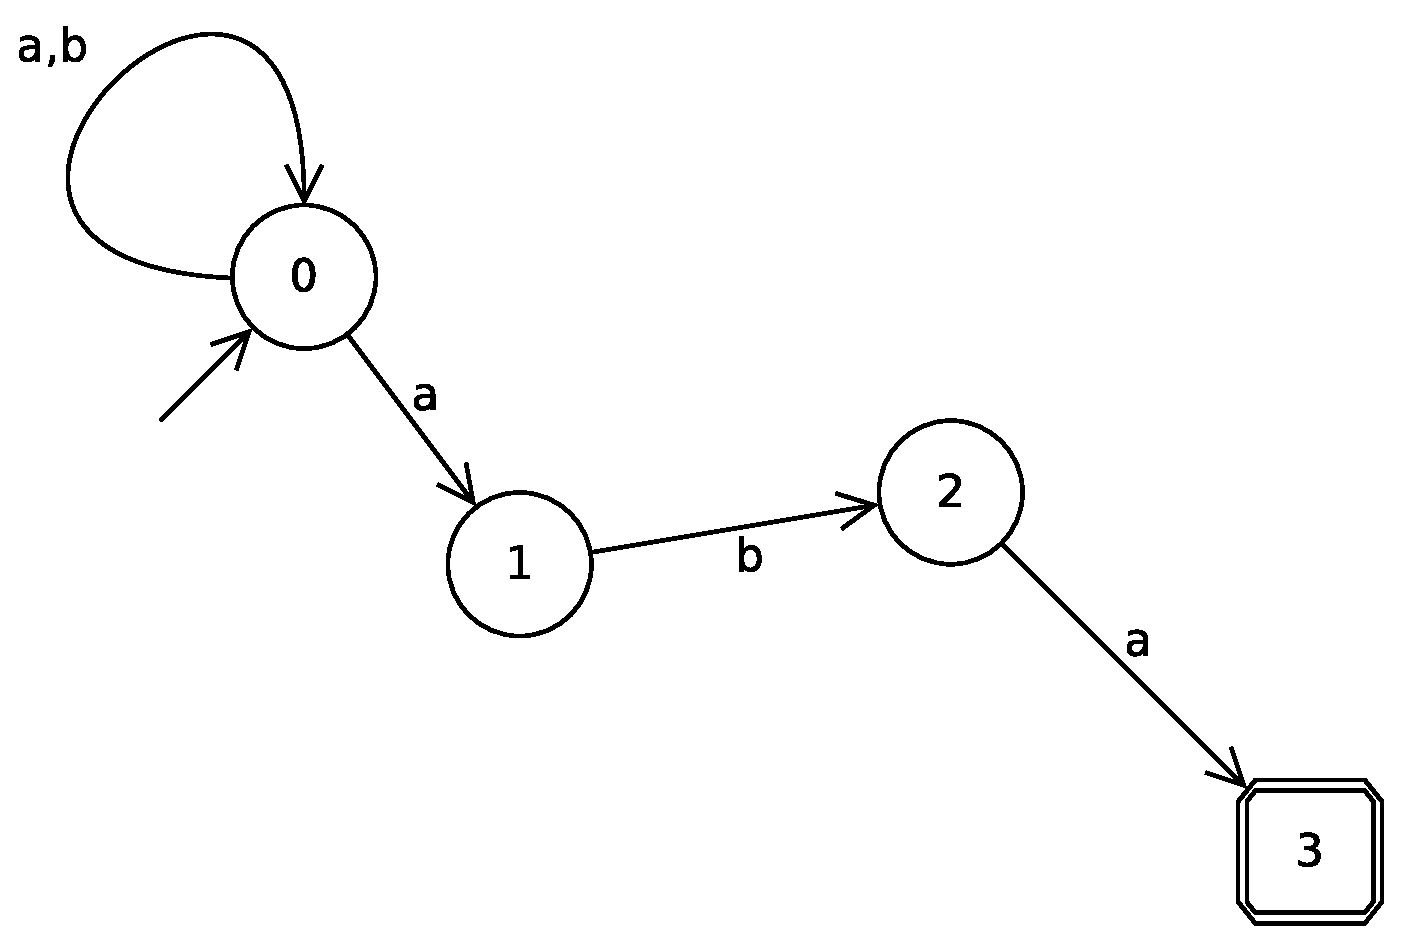
\includegraphics[width=8cm]{images/NFA-1.eps}
	\caption{Ein beispielhafter Automat}
	\label{example_automaton}
\end{figure}

\begin{lstlisting}[caption=Erzeugte XML-Datei,label=example_xml]
<?xml version="1.0" encoding="utf-8"?>
<!DOCTYPE finitestatemachine PUBLIC
  "http://github.com/downloads/wookietreiber
         /scalomator/FiniteStateMachine.dtd">
<finitestatemachine
  xmlns:xsi="http://www.w3.org/2001/XMLSchema-instance"
  xsi:noNamespaceSchemaLocation=
  "http://github.com/downloads/wookietreiber
         /scalomator/FiniteStateMachine.xsd"
  name="foo-o-mat">

  <initialstate>0</initialstate>

  <finalstates>
    <finalstate>3</finalstate>
  </finalstates>

  <transitions>
    <transition>
      <start>0</start>
      <input>a</input>
      <ends>
        <end>0</end>
        <end>1</end>
      </ends>
    </transition>
    <transition>
      <start>0</start>
      <input>b</input>
      <ends>
        <end>0</end>
      </ends>
    </transition>
    <transition>
      <start>1</start>
      <input>b</input>
      <ends>
        <end>2</end>
      </ends>
    </transition>
    <transition>
      <start>2</start>
      <input>a</input>
      <ends>
        <end>3</end>
      </ends>
    </transition>
  </transitions>

</finitestatemachine>

\end{lstlisting}

\end{description}

 \newpage
%  \section{Produktleistungen}

%\comment{Welche zeit- und umfangsbezogenen Anforderungen gibt es?}

\begin{description}
  \item[/L100/]
%    \textit{Schiedsrichter:}
%    Jeder Spieltyp des Systems verf�gt �ber einen eigenen Schiedsrichter, der automatisch erkennt, ob ein Zug g�ltig ist.
%    Zum anderen muss dieser Schiedsrichter erkennen, ob ein Spielende mit dem aktuellen Zug erreicht wurde.
%    Der Schiedsrichter ist kein Mensch, sondern ein Objekt, welches �ber die Regeln des jeweiligen Spieltyps verf�gt.
%  \item[/L200/]
%    \textit{Akkumulation:}
%    Bei fehlererzeugenden Eingaben erh�lt der Benutzer als Fehlermeldung eine Auflistung aller eingegebenen Fehler.
%  \item[/L210/]
%    \textit{Toleranz:}
%    Bei fehlererzeugenden Eingaben muss der Benutzer die M�glichkeit haben, eine Korrektur der Eingabedaten vorzunehmen,
%    ohne Eingaben wiederholt eingeben zu m�ssen.
\end{description}

 \newpage %Produktleistungen erstmal rauslassen?
  \section{Erscheinungsbild}

%\comment{Was sind die grundlegenden Anforderungen an die Benutzungsoberfl�che (Bildschirmlayout, Dialogstruktur, ...)?}


Im Folgenden wird die grobe Struktur des grafischen Benutzeroberfl�che dargestellt.

% hier Bilder von Nils \newpage
  \section{Diagramme}

%hier Klassendiagramm von Christian
\begin{figure}[h!]
	\centering
	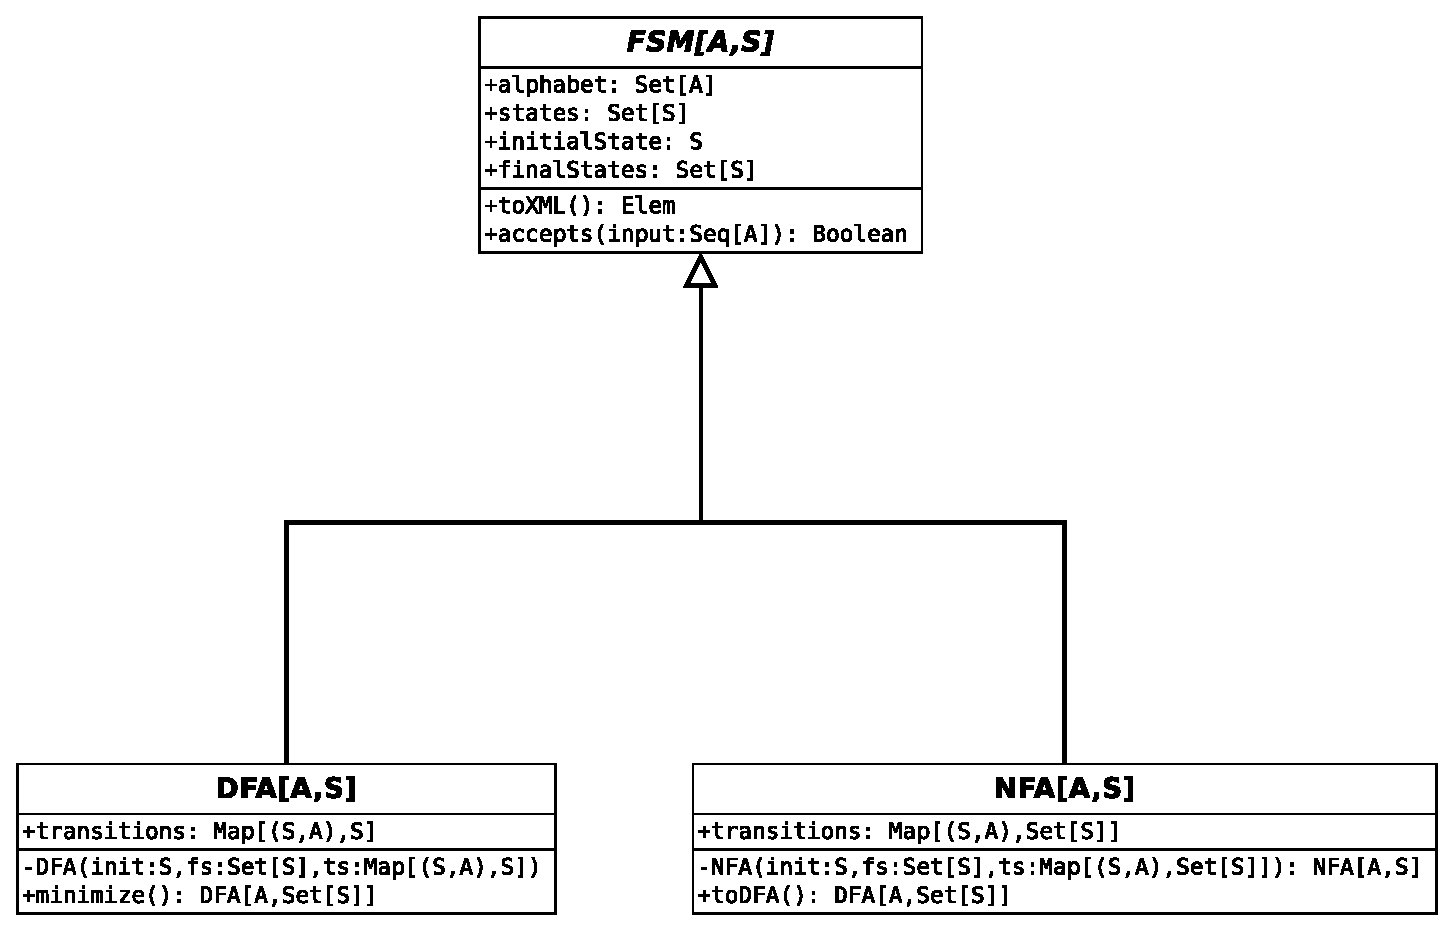
\includegraphics[width=\textwidth]{images/scalomator.eps}
	\caption{Klassendiagramm der Bibliothek}
	\label{class_diagram}
\end{figure}
 \newpage
  \section{Qualit�tszielbestimmungen}

%\comment{Auf welche Qualit�tsanforderungen (Zuverl�ssigkeit, Robustheit, Benutzungsfreundlichkeit, Effizienz, ...) wird besonderen Wert gelegt?}

\begin{center}
 \begin{tabular}{l|c|c|c|c}
  ~ & sehr wichtig & wichtig & weniger wichtig & unwichtig\\
  \hline \hline
  \textit{Robustheit}~ & \textbf{X}~ &  ~ ~ ~ &  ~ ~ ~ &  ~ ~ ~ \\
  \hline
  \textit{Zuverl�ssigkeit}~ & \textbf{X}~ &  ~ ~ ~ &  ~ ~ ~ &  ~ ~ ~ \\
  \hline
  \textit{Korrektheit}~ & \textbf{X}~ &  ~ ~ ~ &  ~ ~ ~ &  ~ ~ ~ \\
  \hline
  \textit{Bedienbarkeit}~ &  ~ ~ ~ & \textbf{X}~ &  ~ ~ ~ &  ~ ~ ~ \\
  \hline
  \textit{Effizienz}~ &  ~ ~ ~ & \textbf{X}~ &  ~ ~ ~ &  ~ ~ ~ \\
  \hline
  \textit{Portabilit�t}~ &  ~ ~ ~ &  ~ ~ ~ & \textbf{X}~ &  ~ ~ ~ \\
  \hline
  \textit{Kompatibilit�t}~ &  ~ ~ ~ &  \textbf{X}~ & ~ ~ ~ &  ~ ~ ~ \\
 \end{tabular}
\end{center}
 \newpage
  \section{Globale Testszenarien und Testf�lle}

Jede Produktfunktion \textit{/F????/} wird anhand von konkreten Testf�llen \textit{/T????/} getestet.\\
Die dabei verwendeten Namen werden rein zuf�llig gew�hlt.

\begin{description}
  \item[/T0010/]
    \textit{Registrieren:}
    Herr Tim Testmann registriert sich mit dem gew�nschten Benutzernamen \textit{testmann}
    und dem Passwort \textit{testtest} und der EMailadresse \textit{tim@testmann.de} am System.\\
    Frau Beate Betamuster registriert sich ebenfall mit dem gew�nschten Benutzernamen \textit{betamuster}
    und dem Passwort \textit{betabeta} und der EMailadresse \textit{info@stefan-baur.de} am System.
  \item[/T0020/]
    \textit{Anmelden:}
    Tim Testmann meldet sich am System unter Benutzung seines Benutzernamens und Passwortes am System an.
  \item[/T0030/]
    \textit{Abmelden:}
    Tim Testmann meldet sich vom System wieder ab.
  \item[/T0040/]
    \textit{Kennung anfordern:}
    Beate Betamuster hat ihre Kennung vergessen und fordert unter Angabe ihrer EMailadresse ihre Kennung an.
  \item[/T0050/]
    \textit{Passwort �ndern:}
    Beate Betamuster �ndert sodann ihr Passwort \textit{betabeta} in \textit{testbeta} ab.
\end{description}
 \newpage
  \section{Entwicklungsumgebung}

%\comment{Welche Software, Hardware und Orgware wird zur Entwicklung ben�tigt?}

Es wird darauf geachtet, dass alle Entwicklungstools kostenfrei sind.

\subsection{Software}

\begin{itemize}
  \item Plattform
    \begin{itemize}
      \item Scala 2.9.1
      \item Java SDK 1.6
      \item GNU/Linux 3.1.6
      \item Windows 7
    \end{itemize}
  \item Tools
    \begin{itemize}
      \item Eclipse Indigo (IDE)
      \item \LaTeX
      \item Texmaker 3.0.2
      \item Scala-IDE f�r Eclipse
      \item Scala Build Tool (SBT)
    \end{itemize}
  \item Versionskontrolle
    \begin{itemize}
      \item git
      \item tortoiseGit
    \end{itemize}
\end{itemize}

\subsection{Hardware}

\begin{itemize}
  \item Laptops / Desktops
\end{itemize}

\subsection{Orgware}

\begin{itemize}
  \item github
\end{itemize}
 \newpage
%  \section{Erg�nzungen}

\comment{Spezielle, noch nicht abgedeckte Anforderungen.}

\subsection{Sprachmodul}
Das System verf�gt �ber ein austauschbares Sprachmodul,
indem alle Texte zum Dialog mit den Benutzern vorliegen und jeweils �ber eine Identifikationsnummer angesprochen werden.\\
Um das System um eine Sprache erweitern zu k�nnen,
muss das Sprachmodul mit der neuen Sprache analog zum bereits existierenen Sprachmodul erstellt werden.
 \newpage %erstmal keine Erg�nzungen
%  \section{Glossar}

%\comment{Definition aller wichtigen Begriffe zur Sicherstellung einer einheitlichen Terminologie.}

\begin{description}
  \item[Automat] Ein Automat ist die Abstraktion eines Rechners, bestehend aus Zust�nden und Zustands�berg�ngen.
  \item[Bibliothek] In der Programmierung ist eine Bibliothek eine Sammlung von Programmfunktionen f�r zusammengeh�rende Aufgaben. Bibliotheken sind im Allgemeinen nicht eigenst�ndig lauff�hig.
  \item[XML] (Extensible Markup Language) ist eine Auszeichnungssprache zur Darstellung hierarchisch strukturierter Daten. XML-Dateien sind Textdateien die zum Austausch von Daten verwendet werden und vom Menschen gelesen werden k�nnen.
  \item[XSD] (XML Schema Definition) definiert die Struktur eines XML-Dokuments. Die XSD-Datei ihrerseits liegt ebenfalls in Form von XML vor.
\end{description}
\end{document}
